\chapter{The problem}
\label{chp:problem}
Given $15$ harmonics of magnetic field measured the high-order corrector superconducting magnets, during a test run, our
objective is to train a machine learning model capable of:
\begin{enumerate}
	\item Recognizing whether the magnet underwent a quench event during operation, we will refer
	      to it as Quench Recognition Problem (\qrp) from now on, and will be treated in
	      \Cref{chp:qrp},
	\item Recognize, if the superconductor quenched, which coil(s) transitioned; we will refer to
	      it as Quench Localization Problem (\qlp) from now on, and it will be treated in
	      \Cref{chp:qlp}.
\end{enumerate}
A field harmonic is a complex function capable of describing the contribution of a certain multipolar
field (e.g. the coefficient associated with the dipole is $C_0$, while $C_1$ is the quadrupolar
coefficient) to the entirety of the magnetic field, which is a vectorial and continuous quantity.

\medskip

This problem, as was already said in previous chapters, is a natural extension of the work done
in~\cite{mariotto2022}~\cite{mariotto2022-generic}, who analyzed the behavior of
a gamma of magnets differing in the number of poles. The original dataset contained the quench
events recorded for every type of magnet, since the number of events for the sole
quadrupoles made up almost the entirety of the dataset we chose to work
exclusively on them.

\medskip

Due to the nature of the problem, we were looking for models that could solve both our problems
while keeping a very high level of explainability. Being able to explain which magnetic field
harmonics are more important to identify reliably a quench event can be of great help in the context of magnet design,
quench explanation and instrument calibration (e.g., \todo{Check with Samuele if this makes sense}\textcolor{blue}{If a new quench antenna needs to be designed the
	researchers know that some magnetic field harmonics can be ignored because they do not influence the
	result}).

\medskip

In the following two sections we will explore the structure of the dataset used for the project and
then we will indicate the instrumentation and processes used to insure the project's
reproducibility.

\section{The datasets and their meaning}
In virtue of the fact that magnetic field harmonics are complex numbers a series of measurements
have been extrapolated, the suffix in the attributes name is related to the number of the considered
harmonic. The meaning of each table is explained briefly here below:
\begin{itemize}
	\item \an: the imaginary part of the magnetic field harmonics;
	\item \bn: the real part of the magnetic field harmonics;
	\item \cnmod: the absolute value of the complex coefficient $C_n$, it's the
	      combination of \an and \bn;
	\item \phin: the phase of the magnetic field harmonics.
\end{itemize}

\section{Model selection and model testing procedures}
Reproducibility is an extremely important property of any experiment, to cover the basics all the
seeds for random number generators were set to the same value. The next step to enforce
reproducibility is using shared pipelines.

Every dataset used in the project is processed using a common pipeline that builds three different
dataframes that are serialized for later reuse:
\begin{itemize}
	\item The \emph{merged} dataframe contains all the field harmonics for a certain table
	      (e.g. \an) or mix of tables (e.g., \an, \bn, \cnmod), before serialization the dataframe is
	      standardized using an instance of the StandardScaler class, contained in scikit-learn, trained
	      on the dataframe just created (minus the label column(s)).
	\item The \emph{safe} dataframe contains a small part of the overall data available to us
	      ($29$ samples), these samples were kept away until the experiments were considered complete.
	      This dataset allowed us to perform a blind test on the best models to see whether they
	      were able to generalize what they previously learned.
	\item The \emph{reduced} dataframe contains the rest of the samples in the original table,
	      it is the main dataframe used to perform tests and experiments.
\end{itemize}

When it came to model selection and model testing we chose to perform a Nested Cross Validation
procedure ($\ncv$). This technique comes with two incredible advantages that suit this problem very
well:
\begin{enumerate}
	\item $\ncv$ is suitable for situations in which the data is not abundant~\cite{Larracy2021} due to the heavy reuse of data during the model selection
	      process, giving also a less biased performance estimation (due to the averaging of
	      the results on more folds),
	\item $\ncv$ is more resilient against overfitting thanks to the 'physical' separation
	      between the hyperparameter selection and testing procedures.
\end{enumerate}
In the following section we will give a brief introduction of the Cross validation procedure.

\subsubsection{Cross Validation}
In \Cref{chp:ml} we talked about the simple train-test splitting procedure, now we will introduce an
alternative technique for splitting that gives us a powerful tool to prevent overfitting and get
less biased performance measures while also doing hyperparameter selection.

\medskip

In general, given a dataset $D$, $k$-fold $\cv$ \cite{ZhouZhi-Hua2021ML} is a technique for splitting a dataset in $k$
different folds $\fold{i}$, the folds are non-overlapping and about the same size, therefore
$\fold{i} \cap \fold{j} = \emptyset \hspace{5pt} \forall i, j \in k$, and the union of all the folds
is the original dataset ($\bigcup_{i \in \{1, \ldots, k\}} \fold{i} = D$).

In the framework of train-test splitting, if we used the procedure introduced in \Cref{chp:ml}, we
would split the original dataset into the training set $T$ and the generalization set $G$, train
$\model$ on $T$ and then test the performance on $G$.

A series of questions normally arise whenever we think about this procedure, we will list them below
and provide an answer.

\medskip

'What if the $T$-$G$ split chosen was the lucky one and the performance we obtain out of the last
reading are overly optimistic?'

\smallskip

This is where $\cv$ comes in, to reduce the probability that the performance of the model
are a statistical anomaly. If we have a dataset of $250$ samples, by doing a
$5$ fold $\cv$, $5$ different folds of $50$ samples are generated, each fold will be used once to
test the generalization performance of the model trained on the remaining $200$ samples.

\medskip

'What value of $k$ should be chosen?'

\smallskip

The number of folds to be used for $\cv$ becomes another hyperparameter of the problem, since it
depends on many factors like the amount of available data, a very big value of $k$ will increase the
number of folds the model is trained and tested on, increasing the robustness of the performance
estimation at the expense of computational complexity (e.g., Leave One Out \cv\ is an example of such
approaches, in~\cite{shao2016} a more efficient approach to the technique is discussed); too small a value of $k$ makes the $\cv$ less
robust but more efficient (classic values of $k$ for most practical uses are $5, 10, 20$).

\medskip

To introduce Nested $\cv$ ($\ncv$) we will consider the case of having to choose the best model,
training it and then testing its performance. In the base case the dataset $D$ can be tripartitioned
as follows:
\begin{itemize}
	\item \emph{Training set} $T$,
	\item \emph{Validation set} $V$, this set of samples will be used to test the performance of the
	      model found after the training step,
	\item \emph{Generalization set} $G$, after the model is retrained on $T + V$ the performance are
	      tested on $G$ to see if the model is capable of generalizing effectively.
\end{itemize}

If we apply this simple procedure to select the model, train it and then test it; how can we
guarantee that the model chosen is the best one, or at least is good enough?

\smallskip

Quite simply, we can't give any guarantees, we might have gotten the worst possible mix of
hyperparameters and still get good performance during the validation and generalization tests due to
statistical anomalies.
\begin{figure}
	\centering
	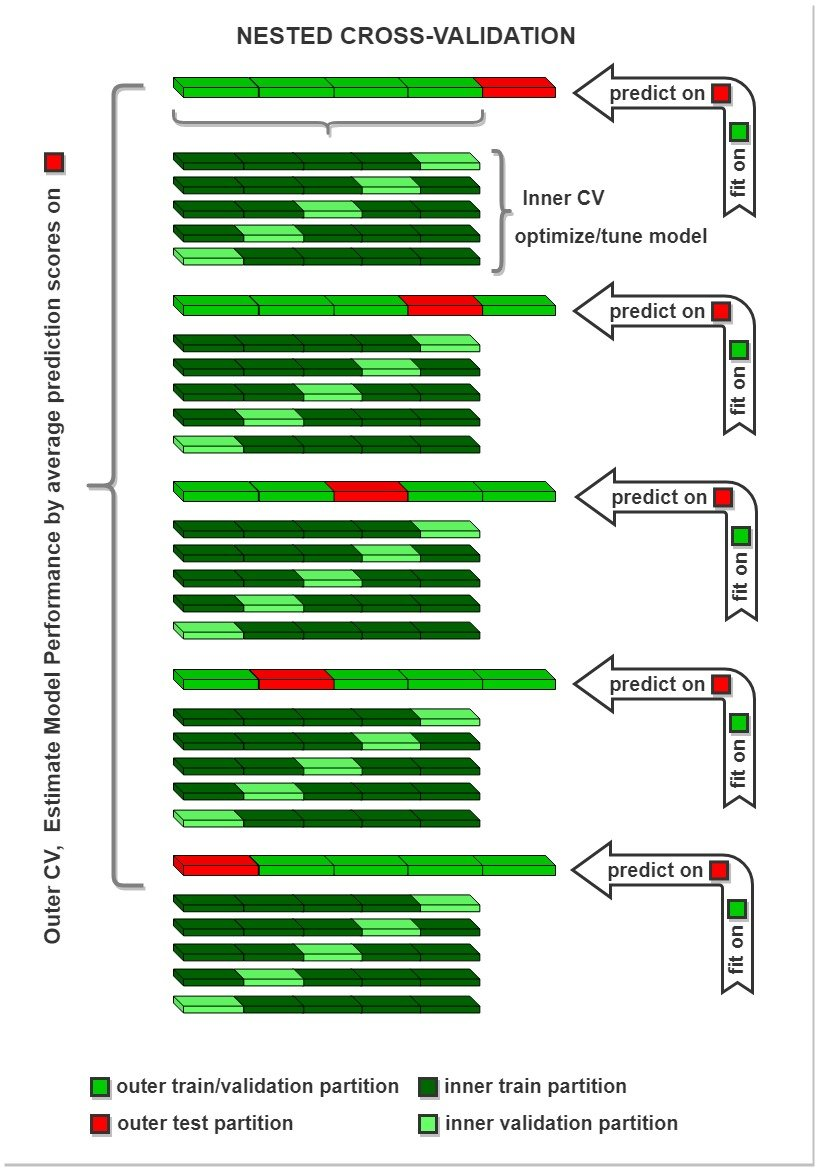
\includegraphics[scale=.3]{./img/nested-cv.png}
	\label{fig:nested-cv}
	\caption{Visualization of the nested cross validation procedure taken from \cite{pain2020}}
\end{figure}
\todo{If I want to add a picture for simple cross validation then something ad hoc should be
	created so that the style is kind of the same}

Compared to the method that we just talked about \ncv, outlined in \Cref{fig:nested-cv}, consists of
two simple \cv\ procedures nested, The outer one is used for testing the generalization performance
of the model, the internal one is used to do model selection and is constructed on the training set
used in the outer loop. Repeating the model selection process gives us better hyperparameter
selection and lowers the chances of us picking a model that performs good only on paper, it also
gives us robust performance estimates since it averages the metrics over different folds.

\medskip

In the project, we chose to apply a $5 \times 5$ \ncv\ procedure, which means that, out of
the $250$ samples that form the original dataset $D$:
\begin{itemize}
	\item The data is first split into $5$ folds of $50$ samples. One fold of $50$ samples will
	      be kept on the side for the generalization test, the remaining $200$ samples will be used to do both training and model selection;
	\item The training set is now split again in $5$ folds, $160$ samples will be used to do
	      model selection (therefore hyperparameter space search), $40$ samples will be used
	      to validate the performance that has been found;
	\item The model found at the previous step is retrained on the whole $200$ training samples and then
	      the performance are tested on the fold that was kept aside in the first step.
\end{itemize}
If we consider once again \Cref{fig:nested-cv} it's clear that the outer \cv\ procedure will yield
$5$ different models, which one should be considered the best model overall? All of the models
obtained after a run of \ncv\ are statistically equivalent, therefore we can pick whichever model we
prefer, usually in practice we keep the model that has the highest accuracy score.

The scikit-learn library contains many \cv\ implementations that can give different or stronger
guarantees compared to the \cv\ procedure shown in this section, the splitting procedure is also
handled differently based on the type of KFold object used.

The closing section for this chapter will contain a summarization of the experiment's
characteristics.
\subsection{Experimental setup}
The project was developed using the latest version of the Python programming language
(3.10.12 at the moment of writing), All experiments have been executed using Python 3.10.12 (the latest version at the time of writing), using the following libraries: scikit-learn (release 1.5.2) for data preprocessing and model training and evaluation, numpy (release 2.2.3) for efficient data storage, and Pandas (release 2.2.3) for data management. These libraries have been handled through the pip package manager (release 25.0.1) and used within a virtual environment.

\medskip

The seeds from the various random number generators have been set to the common value of
\href{https://www.google.com/search?q=the+answer+to+life+the+universe+and+everything&num=10&client=firefox-b-d&sca_esv=a81abf9bb67ffd9b&sxsrf=AHTn8zo6RKep_zuEvIhJb5nuAGh5xAERLg\%3A1739739141586&ei=BVCyZ_C9I9mLi-gP7e-B8Ac&oq=the+answer+to+&gs_lp=Egxnd3Mtd2l6LXNlcnAiDnRoZSBhbnN3ZXIgdG8gKgIIADIIEAAYgAQYywEyCBAAGIAEGMsBMgUQABiABDIIEAAYgAQYywEyCBAAGIAEGMsBMggQABiABBjLATIIEAAYgAQYywEyCBAAGIAEGMsBMggQABiABBjLATIIEAAYgAQYywFIjCJQqQlYiRlwA3gBkAEAmAFuoAHICaoBBDExLjO4AQPIAQD4AQGYAhGgAv0JwgIKEAAYsAMY1gQYR8ICChAjGIAEGCcYigXCAgsQABiABBixAxiDAcICCxAuGIAEGLEDGIMBwgIOEC4YgAQYsQMY0QMYxwHCAg4QLhiABBixAxiDARiKBcICERAuGIAEGLEDGNEDGIMBGMcBwgIMECMYgAQYExgnGIoFwgIEECMYJ8ICDRAuGIAEGEMY1AIYigXCAgoQABiABBhDGIoFwgIOEC4YgAQYxwEYjgUYrwHCAgoQLhiABBhDGIoFwgIIEC4YgAQYsQPCAggQABiABBixA8ICCxAuGIAEGLEDGNQCwgIFEC4YgATCAggQLhiABBjLAcICCxAuGIAEGNEDGMcBmAMAiAYBkAYIkgcEMTIuNaAHrboC&sclient=gws-wiz-serp}{42} to prevent too much deviation in the experiments.

\medskip

The original contained $279$ samples, for \qrp, each sample consisted of $15$ harmonics and a Label
stating whether the sample represents a quench ($1$) event or not ($0$), for \qlp, each sample had $4$ different
labels associated to it representing whether one of the coils ($0$ for East, then: North, West and
South) quenched ($1$) or not ($0$).

Ever splitting operation was performed by stratifying on the labels, in the case of \qlp, if the
labels were more than one, we used a multi-class stratification technique, detailed in (\cite{skmlearn}).

\medskip

Experiments were conducted on three different computers running different architectures and
different operating systems, but the results did not change due to the standard-oriented approach,
\Cref{tbl:computers} for a summary of the computers we used.
\begin{table}[t]
	\caption{System configuration used for our experiments. Core count values are detailed as number
		of CPU cores and threads, while frequency is expressed in the base and boost specifications.
		Finally, the CPU cache size is shown for the L1, L2 and L3 levels, where
		available.}\label{tbl:computers}

	\bigskip

	\centering
	\setlength{\tabcolsep}{4pt}
	\begin{tabular}{lccc}
		\toprule
		                     & \textbf{Pigna}        & \textbf{Mattone}         & \textbf{Topone}    \\
		\midrule
		\textbf{Model}       & Macbook Pro           & Custom build             & Dell XPS 8700      \\
		\textbf{CPU}         & i$5$ $5287\textsc{u}$ & Ryzen 7 $3700\textsc{x}$ & i$7$ $4770$        \\
		\textbf{Core count}  & $2\cc / 2\tc$         & $8\cc / 16\tc$           & $4\cc / 8\tc$      \\
		\textbf{Launch Date} & Q$1$ 2015             & Q$2$ 2019                & Q$2$ 2013          \\
		\textbf{Frequency}   & $2.90 / 3.30$ \ghz    & $4.125 / 4.40$ \ghz      & $3.40 / 3.90$ \ghz \\
		\textbf{Cache}       & $3$ \mb               & $0.512 / 4 / 32$ \mb     & $8$ \mb            \\
		\textbf{TDP}         & $28$ \w               & $84$ \w                  & $65$ \w            \\
		\textbf{RAM}         & $8$ \gb               & $16$ \gb                 & $16$ \gb           \\
		\textbf{OS}          & Pop!\_OS $22.04$ LTS  & Pop!\_OS $22.04$ LTS     & Fedora $39$        \\
		\bottomrule
	\end{tabular}
\end{table}
Experiments were dispatched on different systems based on the expected computational load

Model selection was handled by doing a partial exploration of the parameter space, for each model we
explored a custom parameter grid (shown in \Cref{tbl:params}) via a grid search algorithm (GridSearchCV in scikit-learn).

\begin{table}[t]
	\caption{Hyperparameters which we have tuned during the model training phase.} \label{tbl:params}

	\bigskip

	\centering
	\setlength{\tabcolsep}{6pt}
	\begin{tabular}{llc}
		\toprule
		\textbf{Model}       & \textbf{Hyperparameter}                                           & \textbf{Values}                        \\
		\midrule
		\multirow{5}{*}{DT}  & impurity criterion                                                & gini, entropy, log loss                \\
		                     & max depth                                                         & $2, 3, 4, 5$                           \\
		                     & min impurity decrease                                             & $0.001, 0.01, 0.05$                    \\
		                     & max features                                                      & None, $0.5, 0.75$                      \\
		                     & min samples leaf                                                  & $5, 10, 20$                            \\
		\midrule
		\multirow{1}{*}{RF}  & n. of trees                                                       & $2, 3, 5, 10$                          \\
		                     & \multicolumn{2}{l}{$+$ the same hyperparameters and values of DT}                                          \\
		\midrule
		\multirow{5}{*}{SVC} & $C$                                                               & $0.1, 1, 10, 100, 1000$                \\
		                     & $\gamma$                                                          & scale, auto, $0.001, 0.01, 0.1, 1, 10$ \\
		                     & degree                                                            & $2, 3, 4, 5$                           \\
		                     & $c_0$                                                             & $0, 0.1, 0.5, 1$                       \\
		                     & kernel                                                            & linear, poly sigmoid, rbf              \\
		\bottomrule
	\end{tabular}
\end{table}







